\documentclass[Chap2main.tex]{subfiles}

% Load any packages needed for this document

\begin{document}
	\section{Limits of Agreement}
	% introduces
	A third element of the Bland-Altman methodology, an interval known
	as `limits of agreement' is introduced in \citet*{BA86}
	(sometimes referred to in literature as 95\% limits of agreement).
	Limits of agreement are used to assess whether the two methods of
	measurement can be used interchangeably. \citet{BA86} refer to
	this as the `equivalence' of two measurement methods. The specific purpose of the limits of
	agreement must be
	established clearly. \citet*{BA95} comment that the limits of agreement `how
	far apart measurements by the two methods were likely to be for
	most individuals', a definition echoed in their 1999 paper:
	
	\begin{quote}"We can then say that nearly all pairs
		of measurements by the two methods will be closer together than
		these extreme values, which we call 95\% limits of agreement.
		These values define the range within which most differences
		between measurements by the two methods will lie."
	\end{quote}
	
	The limits of agreement (LoA) are computed by the following
	formula:
	\[
	LoA = \bar{d} \pm 1.96 s_{d}
	\]
	with $\bar{d}$ as the estimate of the inter method bias, $s_{d}$
	as the standard deviation of the differences and 1.96 is the 95\%
	quantile for the standard normal distribution. (Some accounts of
	Bland-Altman plots use a multiple of 2 standard deviations instead
	for simplicity.)
	
	The limits of agreement methodology assumes a constant level of bias throughout the range of measurements. Importantly the authors recommend prior determination of what would and would constitute acceptable
	agreement, and that sample sizes should be predetermined to give an accurate conclusion. However \citet{mantha} highlights inadequacies in the correct application of limits of agreement, resulting in contradictory estimates limits of agreement in various papers.
	
	\begin{quote}
		``How far apart measurements can be without causing difficulties
		will be a question of judgment. Ideally, it should be defined in
		advance to help in the interpretation of the method comparison and
		to choose the sample size \citep{BA86}".
	\end{quote}
	
	
	For the Grubbs `F vs C' comparison, these limits
	of agreement are calculated as -0.132 for the upper bound, and
	-1.08 for the lower bound. Figure 1.9 shows the resultant
	Bland-Altman plot, with the limits of agreement shown in dashed
	lines.
	
	
	\begin{figure}[h!]
		\begin{center}
			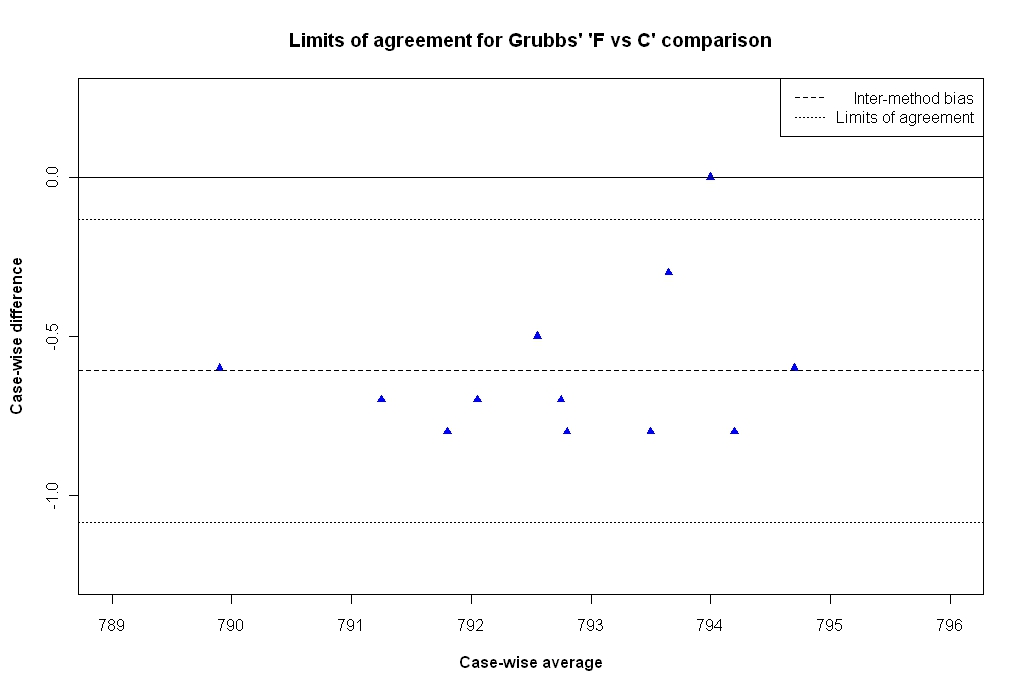
\includegraphics[width=125mm]{GrubbsBAplot-LOA.jpeg}
			\caption{Bland-Altman plot with limits of agreement}\label{GrubbsBAplot-noLOA}
		\end{center}
	\end{figure}
	
	%But as \citet*{BA86} point out this may not be the case. Variants of the limits of agreement that overcome this
	% problem shall be introduced in due course.
	
	
	\subsection{Formal definition of limits of agreement}
	\citet{BA99} note the similarity of limits of agreement to
	confidence intervals, but are clear that they are not the same
	thing. Interestingly, they describe the limits as `being like a
	reference interval'.
	
	Limits of agreement have very similar construction to Shewhart
	control limits. The Shewhart chart is a well known graphical
	methodology used in statistical process control. Consequently
	there is potential for misinterpreting the limits of agreement as
	if equivalent to Shewhart control limits. Importantly the
	parameters used to determine the Shewhart limits are not based on any sample used for an analysis, but
	on the process's historical values, a key difference with
	Bland-Altman limits of agreement.
	
	\citet{BXC2008} regards the limits of agreement as a prediction
	interval for the difference between future measurements with the
	two methods on a new individual, but states that it does not fit
	the formal definition of a prediction interval, since the
	definition does not consider the errors in estimation of the
	parameters. Prediction intervals, which are often used in
	regression analysis, are estimates of an interval in which future
	observations will fall, with a certain probability, given what has
	already been observed. \citet{BXC2008} offers an alternative
	formulation, a $95\%$ prediction interval for the difference
	\[
	\bar{d} \pm t_{(0.975, n-1)}s_{d} \sqrt{1+\frac{1}{n}}
	\]
	
	\noindent where $n$ is the number of subjects. Carstensen is
	careful to consider the effect of the sample size on the interval
	width, adding that only for 61 or more subjects is there a
	quantile less than 2.
	
	\citet{luiz} offers an alternative description of limits of
	agreement, this time as tolerance limits. A tolerance interval for
	a measured quantity is the interval in which a specified fraction
	of the population's values lie, with a specified level of
	confidence. \citet{Barnhart} describes them as a probability
	interval, and offers a clear description of how they should be
	used;`if the absolute limit is less than an acceptable difference
	$d_{0}$, then the agreement between the two methods is deemed
	satisfactory'.
	
	The prevalence of contradictory definitions of what limits of agreement strictly are will inevitably attenuate the poor standard of reporting using limits of agreement, as mentioned by \citet{mantha}.
	
	%At least 100 historical
	%values must be used to determine the acceptable value (i.e the
	%process mean) and the process standard deviation. The principle
	%that the mean and variance of a large sample of a homogeneous
	%population is a close approximation of the population's mean and
	%variance justifies this.
	
	%\begin{figure}[h!]
	%\begin{center}
	%  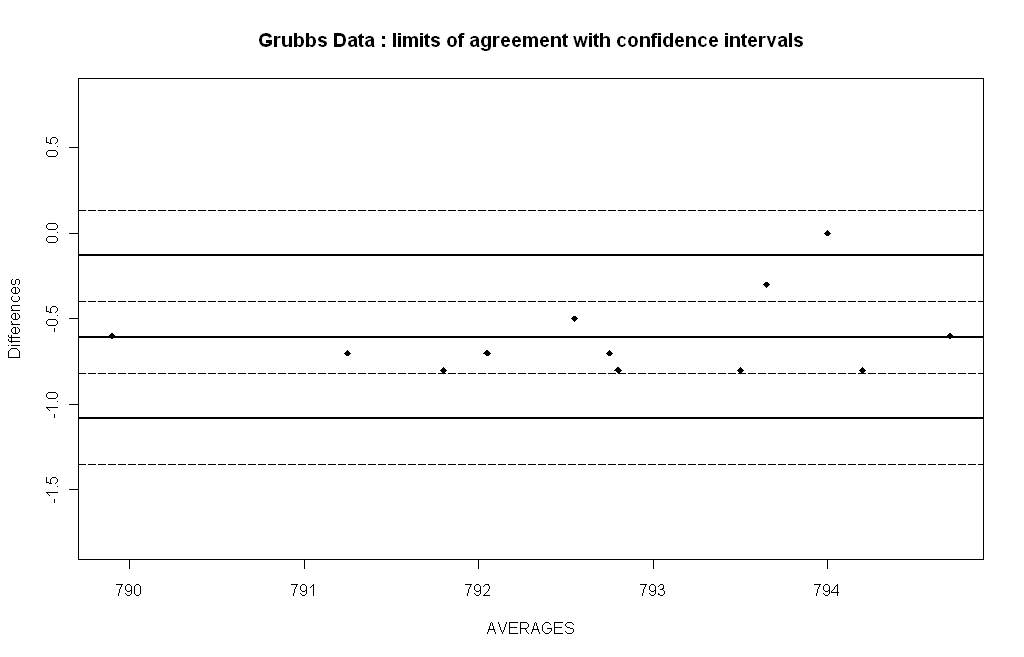
\includegraphics[width=125mm]{GrubbsLOAwCIs.jpeg}
	%  \caption{Limits of agreement with confidence intervals}\label{LOAwCIs}
	%\end{center}
	%\end{figure}
	
	%\newpage
	%\section{Agreement Indices}
	%\citet{Barnhart} provided an overview of several agreement
	%indices, including the limits of agreement. Other approaches, such
	%as mean squared deviation, the tolerance deviation index and
	%coverage probability are also discussed.
	
	
	
	
	\subsection{Replicate Measurements}
	
	Thus far, the formulation for comparison of two measurement
	methods is one where one measurement by each method is taken on
	each subject. Should there be two or more measurements by each
	methods, these measurement are known as `replicate measurements'.
	\citet{BXC2008} recommends the use of replicate measurements, but
	acknowledges the additional computational complexity.
	
	\citet*{BA86} address this problem by offering two different
	approaches. The premise of the first approach is that replicate
	measurements can be treated as independent measurements. The
	second approach is based upon using the mean of the each group of
	replicates as a representative value of that group. Using either
	of these approaches will allow an analyst to estimate the inter
	method bias.
	
	%\subsubsection{Mean of Replicates Limits of Agreement}
	
	However, because of the removal of the effects of the replicate
	measurements error, this would cause the estimation of the
	standard deviation of the differences to be unduly small.
	\citet*{BA86} propose a correction for this.
	
	\citet{BXC2008} takes issue with the limits of agreement based on
	mean values of replicate measurements, in that they can only be interpreted as prediction
	limits for difference between means of repeated measurements by
	both methods, as opposed to the difference of all measurements.
	Incorrect conclusions would be caused by such a misinterpretation.
	\citet{BXC2008} demonstrates how the limits of agreement
	calculated using the mean of replicates are `much too narrow as
	prediction limits for differences between future single
	measurements'. This paper also comments that, while treating the
	replicate measurements as independent will cause a downward bias
	on the limits of agreement calculation, this method is preferable
	to the `mean of replicates' approach.
	
	
	\subsection{Bland-Altman correlation test}
	
	The approach proposed by \citet{BA83} is a formal test on the
	Pearson correlation coefficient of case-wise differences and means
	($\rho_{AD}$). According to the authors, this test is equivalent
	to the `Pitman Morgan Test'. For the Grubbs data, the correlation
	coefficient estimate ($r_{AD}$) is 0.2625, with a 95\% confidence
	interval of (-0.366, 0.726) estimated by Fishers `$r$ to $z$'
	transformation \citep*{Cohen}. The null hypothesis ($\rho_{AD}$ =0)
	fail to be rejected. Consequently the null hypothesis of equal
	variances of each method would also fail to be rejected. There has
	no been no further mention of this particular test in
	\citet{BA86}, although \citet{BA99} refers to Spearman's rank
	correlation coefficient. \citet{BA99} comments `we do not see a
	place for methods of analysis based on hypothesis testing'.
	\citet{BA99} also states that consider structural equation models
	to be inappropriate.
	
	\subsection{Identifiability}
	\citet{DunnSEME} highlights an important issue regarding using
	models such as these, the identifiability problem. This comes as a
	result of there being too many parameters to be estimated.
	Therefore assumptions about some parameters, or estimators used,
	must be made so that others can be estimated. For example in literature the variance
	ratio $\lambda=\frac{\sigma^{2}_{1}}{\sigma^{2}_{2}}$
	must often be assumed to be equal to $1$ \citep{linnet98}.\citet{DunnSEME} considers methodologies based on two methods with single measurements on each subject as inadequate for a serious
	study on the measurement characteristics of the methods. This is
	because there would not be enough data to allow for a meaningful
	analysis. There is, however, a contrary argument that in many
	practical settings it is very difficult to get replicate
	observations when the measurement method requires invasive medical
	procedure.
	
	%%%%%%%%%%%%%%%%%%%%%%%%%%%%%%%%%%%%%%%%%%%%%%%%%%%%%%%%%%%%%%%%%%%%%%%%%%%%%%%Bartko's BB
	\citet{BB89} offers a formal simultaneous hypothesis test for the
	mean and variance of two paired data sets. Using simple linear
	regression of the differences of each pair against the sums, a
	line is fitted to the model, with estimates for intercept and
	slope ($\hat{\beta}_{0}$ and $\hat{\beta}_{1}$). The null
	hypothesis of this test is that the mean ($\mu$) and variance
	($\sigma^{2}$) of both data sets are equal if the slope and
	intercept estimates are equal to zero(i.e $\sigma^{2}_{1} =
	\sigma^{2}_{2}$ and $\mu_{1}=\mu_{2}$ if and only if $\beta_{0}=
	\beta_{1}=0$ )
	
	A test statistic is then calculated from the regression analysis
	of variance values \citep{BB89} and is distributed as `$F$' random
	variable. The degrees of freedom are $\nu_{1}=2$ and $\nu_{1}=n-2$
	(where $n$ is the number of pairs). The critical value is chosen
	for $\alpha\%$ significance with those same degrees of freedom.
	\citet{Bartko} amends this methodology for use in method
	comparison studies, using the averages of the pairs, as opposed to
	the sums, and their differences. This approach can facilitate
	simultaneous usage of test with the Bland-Altman methodology.
	Bartko's test statistic take the form:
	\[ F.test = \frac{(\Sigma d^{2})-SSReg}{2MSReg}
	\]
	% latex table generated in R 2.6.0 by xtable 1.5-5 package
	% Mon Aug 31 15:53:51 2009
	\begin{table}[ht]
		\begin{center}
			\begin{tabular}{lrrrrr}
				\hline
				& Df & Sum Sq & Mean Sq & F value & Pr($>$F) \\
				\hline
				Averages & 1 & 0.04 & 0.04 & 0.74 & 0.4097 \\
				Residuals & 10 & 0.60 & 0.06 &  &  \\
				\hline
			\end{tabular}
			\caption{Regression ANOVA of case-wise differences and averages
				for Grubbs Data}
		\end{center}
	\end{table}
	%(calculate using R code $qf(0.95,2,10)$).
	
	For the Grubbs data, $\Sigma d^{2}=5.09 $, $SSReg = 0.60$ and
	$MSreg=0.06$ Therefore the test statistic is $37.42$, with a
	critical value of $4.10$. Hence the means and variance of the
	Fotobalk and Counter chronometers are assumed to be simultaneously
	equal.
	
	Importantly, this methodology determines whether there is both
	inter-method bias and precision present, or alternatively if there
	is neither present. It has previously been demonstrated that there
	is a inter-method bias present, but as this procedure does not
	allow for separate testing, no conclusion can be drawn on the
	comparative precision of both methods.
	
	
	
	%This application of the
	%Grubbs method presumes the existence of this condition, and necessitates
	%replication of observations by means external to and independent of the first
	%means. The Grubbs estimators method is based on the laws of propagation of
	%error. By making three independent simultaneous measurements on the same
	%physical material, it is possible by appropriate mathematical manipulation of
	%the sums and differences of the associated variances to obtain a valid
	%estimate of the precision of the primary means. Application of the Grubbs
	%estimators procedure to estimation of the precision of an apparatus uses
	%the results of a physical test conducted in such a way as to obtain a series
	%of sets of three independent observations.
	
	
	\section{Regression Methods}
	Conventional regression models are estimated using the ordinary
	least squares (OLS) technique, and are referred to as `Model I
	regression' \citep{CornCoch,ludbrook97}. A key feature of Model I
	models is that the independent variable is assumed to be measured
	without error. As often pointed out in several papers
	\citep{BA83,ludbrook97}, this assumption invalidates simple linear
	regression for use in method comparison studies, as both methods
	must be assumed to be measured with error.
	
	The use of regression models that assumes the presence of error in
	both variables $X$ and $Y$ have been proposed for use instead
	\citep{CornCoch,ludbrook97}. These methodologies are collectively
	known as `Model II regression'. They differ in the method used to
	estimate the parameters of the regression.
	
	Regression estimates depend on formulation of the model. A
	formulation with one method considered as the $X$ variable will
	yield different estimates for a formulation where it is the $Y$
	variable. With Model I regression, the models fitted in both cases
	will entirely different and inconsistent. However with Model II
	regression, they will be consistent and complementary.
	
	Regression approaches are useful for a making a detailed examination of the biases across the range of measurements, allowing bias to be decomposed into fixed bias and proportional bias.
	Fixed bias describes the case where one method gives values that are consistently different
	to the other across the whole range. Proportional
	bias describes the difference in measurements getting progressively greater, or smaller, across the range of measurements. A measurement method may have either an attendant fixed bias or proportional bias, or both. \citep{ludbrook}. Determination of these biases shall be discussed in due course.
	
	\section{Limits of Agreement}
	
	Computing limits of agreement features prominently in many method comparison studies, further to \citet{BA86,BA99}.
	\citet{BA99} addresses the issue of computing LoAs in the presence of replicate measurements, suggesting several computationally simple approaches. When repeated measures data are available, it is desirable to use
	all the data to compare the two methods. However, the original Bland-Altman method was developed for two sets of measurements done on one occasion (i.e. independent data), and so this approach is not suitable for replicate measures data. However, as a naive analysis, it may be used to explore the data because of the simplicity of the method.
	\citet{bxc2008}  computes the limits of agreement to the case with replicate measurements by using LME models.
	
	\section{Outline of Thesis}
	Thus the study of method comparison is introduced. The intention of this thesis is to progress the
	study of method comparison studies, using a statistical method known as Linear mixed effects models.
	Chapter two shall describe linear mixed effects models, and how the use of the linear mixed
	effects models have so far extended to method comparison studies. Implementations of important existing work shall be presented, using the \texttt{R} programming language.
	
	Model diagnostics are an integral component of a complete statistical analysis.
	In chapter three model diagnostics shall be described in depth, with particular
	emphasis on linear mixed effects models, further to chapter two.
	
	For the fourth chapter, important linear mixed effects model diagnostic methods shall be extended to method comparison studies, and proposed methods shall be demonstrated on data sets that have become well known in literature on method comparison. The purpose is to both calibrate these methods and to demonstrate applications for them.
	The last chapter shall focus on robust measures of important parameters such as agreement.
	
	\bibliography{DB-txfrbib}
\end{document}
